\newpage
\fancyfoot[LO,RE]{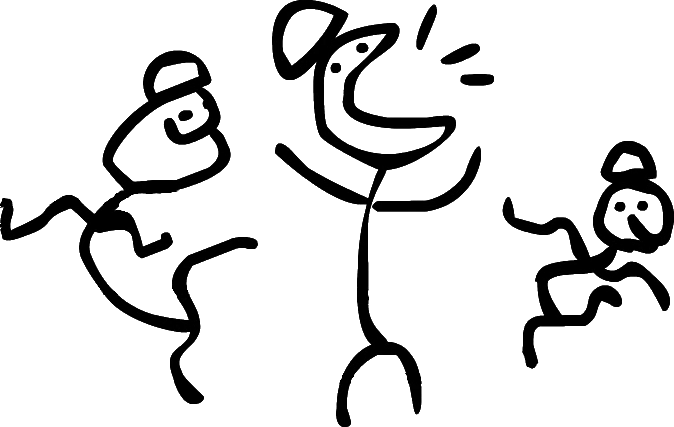
\includegraphics[height=45pt]{images/hutnicy.png}}
\begin{song}{title={Piosenka o hucie}, lyrics={Jakub \say{Dem3000} Dębski}, music={Romek Buga}, capo=1, annex}
    \begin{intro}
        \say{Czasami w hu^{Dmaj7}cie spotykamy się wszyscy i pracujemy tam \\
        A ^{e7}czasami nie, czasami śpiewamy piosenki, na przykład moją ulubio-- \\
        Moją ^{A7}ulubioną piosenkę} --- pomyślał sobie, przypomniał sobie swoją ulubioną piosenkę:
    \end{intro}
    \begin{chorus}
        ^{Dmaj7}Hej! ^*{h7} Otrzymy ^{e7}wanie me^{A7}tali \\
        Z r^{Dmaj7}ud i z^{h7}łomu ^{e7} ^{A7} \\
        To jest ^{Dmaj7}to, co ^{h7}lubię naj^{e7}bardziej ^{A7} \\
        To jest ^{Dmaj7}to, co ^{h7}lubię naj^{e7}bardziej \\
        ^{A7}Wytapiać sz^{Dmaj7}kło --- i prze^{h7}twarzać produkty sz^{e7}klane ^{A7} \\
        Praca w ^*{Dmaj7}hu--- ^*{h7}uc ^{e7}ie ^{A7} \\
        Praca w hu^{Dmaj7}cie
    \end{chorus}
\end{song}

